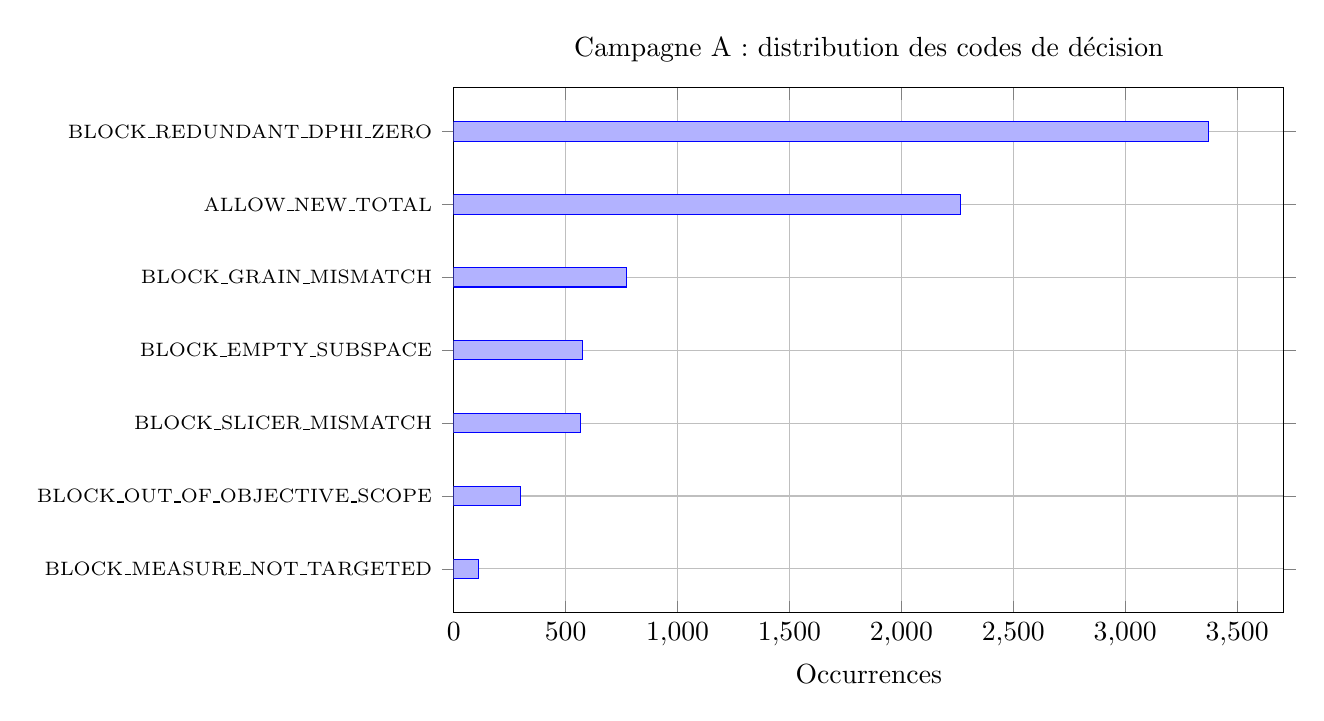
\begin{tikzpicture}
\begin{axis}[xbar,
bar width=7pt,
width=\linewidth,
height=0.68\linewidth,
title={Campagne A : distribution des codes de décision},
xlabel={Occurrences},
ytick={0,1,2,3,4,5,6},
yticklabels={{BLOCK\_MEASURE\_NOT\_TARGETED},{BLOCK\_OUT\_OF\_OBJECTIVE\_SCOPE},{BLOCK\_SLICER\_MISMATCH},{BLOCK\_EMPTY\_SUBSPACE},{BLOCK\_GRAIN\_MISMATCH},{ALLOW\_NEW\_TOTAL},{BLOCK\_REDUNDANT\_DPHI\_ZERO}},
y tick label style={font=\scriptsize},
grid=major,
xmin=0]
\addplot+ coordinates {(110,0) (300,1) (566,2) (576,3) (770,4) (2266,5) (3372,6)};
\end{axis}
\end{tikzpicture}
